\documentclass{ldr-simple-gray}


%------------------------------------------------------------
%首页start
\title{基于稀疏图码的离群值去除}

\subtitle{本科毕业论文(设计)答辩}

\author{庄启源}

\institute[]
{
导师:李朋\quad 副教授\\
% 记得改啊,老是有人不改学院……
兰州大学\quad 数学与统计学院
}

\date{\today}

% \logo{
\includegraphics[height=1cm]{lzu_logo.png}}
\titlegraphic{
\includegraphics[height=1.5cm]{lzu_logo.png}}

%首页end
%------------------------------------------------------------

\begin{document}

%封面
\frame{\titlepage}


\begin{frame}{个人信息}

    \begin{itemize}
        % 记得改啊
        \item 姓名:庄启源
        \item 导师:李朋 副教授
        \item 专业:数学(基础理论班)
    \end{itemize}

    \qquad \noindent\rule[0.25\baselineskip]{0.9\textwidth}{1pt}

    \begin{itemize}
        \item 本科:2016-2020 \quad 兰州大学 \quad 物理科学与技术学院
        \item 硕士:2020-至今 \quad 兰州大学 \quad 物理科学与技术学院
    \end{itemize}

    \qquad \noindent\rule[0.25\baselineskip]{0.9\textwidth}{1pt}

    \begin{itemize}
        \item 已发表文章:梦里什么都有 ~
    \end{itemize}
\end{frame}

% 要把今天讲的研究背景、主要结果、价值和意义(贡献点)讲清楚

\section{研究背景}

\begin{frame}{相关解释}
    \begin{itemize}
        \item 注意字体,默认很丑,请自行设置,在ldr-simple-gray.cls文件里,注释掉了
        \item 适用于兰州大学,任何时候
        \item 比如:本科、研究生、硕士等毕业答辩
        \item 比如:转博士、组会等任何时候
        \item 尤其是组会、方便以后写论文时找找找
    \end{itemize}
    
\end{frame}


\begin{frame}{现有研究}
    答辩中参考文献放在每页下面,方便应对提问:比如年限、作者、期刊等
    \begin{figure}
        \subfigure[2nm、10-160\%\footfullcite{Zhang2011}]{
            
\includegraphics[width=0.28\textwidth]{lammps.png}
         }
         \subfigure[5nm、50-350\%\footfullcite{Zhang2011}]{
             
\includegraphics[width=0.36\textwidth]{lammps.png}
          }\\
        \subfigure[20nm、25-45\%\footfullcite{Zhang2011}]{
            
\includegraphics[width=0.4\textwidth]{lammps.png}
         }
    \end{figure}
\end{frame}


\begin{frame}{存在的问题}
    
    \begin{itemize}
        \item 你的独特点与创新是什么?
        \item 概括、分条
    \end{itemize}
\end{frame}

\section{研究内容}

\begin{frame}{做了啥?}
    复杂布局:上下布局、左右分栏

    \begin{columns}
        \column{0.7\textwidth}
    \begin{itemize}
        \item 11111
        \item 22222
        \item 33333
    \end{itemize}

    \begin{figure}
        
\includegraphics[width=0.4\textwidth]{lammps.png}
        \caption{图图图}
    \end{figure}
    \column{0.3\textwidth}

    \begin{figure}
        
\includegraphics[angle=80, width=0.4\textwidth]{lammps.png}
        \caption{我转}
    \end{figure}

\end{columns}

\end{frame}


\begin{frame}{价值和意义}
    
    \begin{itemize}
        \item 给出了……,预测了……。
        \item 相比其他,此材料\textcolor{Logo2}{多厉害、多厉害、……}
        \item 为……提供了解决思路。
    \end{itemize}
    
\end{frame}

\section{博士计划}

\begin{frame}{计划往往是不去做、或无法完成的}

    找女朋友,找女朋友,找女朋友\footfullcite{Zhang2011}

    找女朋友,找女朋友,找女朋友\footfullcite{Zhang2011}

    找女朋友,找女朋友,找女朋友\footfullcite{Zhang2011}

    \begin{figure}[H]
        \centering
        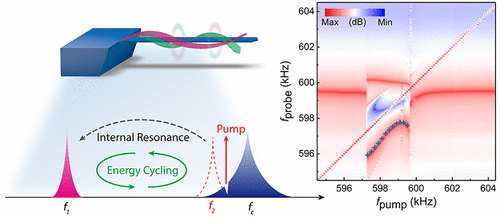
\includegraphics[width=0.47\textwidth]{2022-04-16-06-26-14.png}
    \end{figure}
    重要的事情说9遍,九九归一、大彻大悟

\end{frame}


\begin{frame}{\quad}
\begin{center}
       \zihao{2} 谢\quad 谢!
\end{center}

\end{frame}

\end{document}